\documentclass{"../../res/univ-projet"}
\usepackage[latin1]{inputenc}
\usepackage{array}
\usepackage[T1]{fontenc}
\usepackage[francais]{babel}

\title{Sp\'{e}cification Technique des Besoins}
\author{\bsc{Michotte} Maxime}
\projet{M1SSI}
\projdesc{Projet de g\'{e}n\'{e}ration d'OTP}
\filiere{M1SSI}
\version{1.0}
\relecteur{\bsc{Zigh} Benjamin}
\signataire{\bsc{Bardet} Magali}
\date{Novembre 2013}

\histentry{1.0}{15/11/2013}{Version initiale.}
\histentry{1.1}{28/11/2013}{Ajout terminologie et modification sch\'{e}ma sch�ma}

\begin{document}
\maketitle
%-------------------------------------------------------------------------------
\section{Objet}
Etude et impl\'{e}mentations des syst�mes d'authentification utilisant des mots de passe jetables :
\begin{itemize}
    \item Besoins op\'{e}rationnels
        \begin{itemize}
            \item Garantir une authentification forte
            \item Etat de l'art sur les syst�mes existants
            \item Objectif : mise en production
        \end{itemize}
    \item Objectifs techniques
    \begin{itemize}	
            \item Impl\'{e}mentation des solutions retenues sur un ou plusieurs supports
    \end{itemize}
    \item Contraintes et recommandations
        \begin{itemize}
            \item Respecter les sp\'{e}cifications de base et les normes RFC
            \item Montrer que le syst�me produit est s�r
            \item Choisir une impl\'{e}mentation adapt\'{e}e en fonction des besoins et de l'\'{e}tat de l'art \'{e}tabli
        \end{itemize}
    \item R\'{e}sultats attendus
        \begin{itemize}
            \item Syst�me s�r et fonctionnel
            \item Etat de l'art le plus exhaustif possible
            \item Impl\'{e}mentation sur Carte � puces et/ou Android
        \end{itemize}
\end{itemize}
%-------------------------------------------------------------------------------
\section{Documents applicables et de r�f�rence}

\begin{tabular}{p{1,5cm}>{\raggedright\arraybackslash}p{13cm}}
{[ANS10]} & {ANSSI. R\'{e}f\'{e}rentiel g\'{e}n\'{e}ral de s\'{e}curit\'{e}. \href{http://www.ssi.gouv.fr/fr/reglementation-ssi/referentiel-general-de-securite}{http://www.ssi.gouv.fr/fr/reglementation-ssi/referentiel-general-de-securite}, 2010.}
\tabularnewline
\\
{[MvOV97]} & {Alfred J. Menezes, Paul C. van Oorschot, and Scott A. Vanstone. Handbook of applied cryptography. CRC Press Series on Discrete Mathematics and its Applications. CRC Press, Boca Raton, FL, 1997. With a foreword by Ronald L.Rivest.}
\tabularnewline
\\
{[RFC98]} & {A One-Time Password System. \href{http://tools.ietf.org/html/rfc2289}{http://tools.ietf.org/html/rfc2289}, 1998.}
\tabularnewline
\\
{[RFC05]} & {HOTP:An HMAC-Based One-Time Password Algorithm \href{http://tools.ietf.org/html/rfc4226}{http://tools.ietf.org/html/rfc4226}, 2005.}
\tabularnewline
\\
{[RFC06]} & {Generic Message Exchange Authentication for the Securer Shell Protocol (SSH).\href{http://tools.ietf.org/html/rfc4256}{http://tools.ietf.org/html/rfc4256}, 2006.}
\tabularnewline
\\
{[RFC07]} & {The EAP Protected One-Time Password Protocol (EAP-POTP). \href{http://tools.ietf.org/html/rfc4793}{http://tools.ietf.org/html/rfc4793}, 2007.}
\tabularnewline
\\
{[RFC11]} & {TOTP: Time-Based One-Time Password Algorithm \href{http://tools.ietf.org/html/rfc6238}{http://tools.ietf.org/html/rfc6238}, 2011.}
\tabularnewline
\\
{[goo]} & {Google Authentificator \href{https://code.google.com/p/google-authenticator/}{https://code.google.com/p/google-authenticator/}.}
\tabularnewline
\\
\end{tabular}
\newpage
%-------------------------------------------------------------------------------
\section{Terminologie et sigles utilis�s}
\begin{itemize}
\item \textbf{Etat de l'art}\\
  Dresser un \'{e}tat de l'art dans un domaine consiste � rechercher toutes les informations existantes concernant ce domaine et � en faire une synth�se.

\item \textbf{RFC}\\
  Les RFC (Request For Comments) sont un ensemble de documents qui font r\'{e}f\'{e}rence aupr�s de la Communaut\'{e} Internet et qui d\'{e}crivent, sp\'{e}cifient, aident � l'impl\'{e}mentation, standardisent et d\'{e}battent de la majorit\'{e} des normes, standards, technologies et protocoles li\'{e}s � Internet et aux r\'{e}seaux en g\'{e}n\'{e}ral.

\item \textbf{Utilisateur}\\
  L'utilisateur est une personne physique qui dans notre cas souhaite utiliser une authentification utilisant les OTP.

\item \textbf{Mot de passe}\\
  Le mot de passe est une m\'{e}thode parmi d'autres pour effectuer une authentification, c'est-�-dire v\'{e}rifier qu'une personne correspond bien � l'identit\'{e} d\'{e}clar\'{e}e. Il s'agit d'une preuve que l'on poss�de et que l'on transmet au service charg\'{e} d'autoriser l'acc�s. Le mot de passe doit �tre tenu secret pour \'{e}viter qu'un tiers non autoris\'{e} puisse acc\'{e}der � la ressource ou au service.  
  
\item \textbf{OTP}\\
  Un Mot de passe unique ou OTP (One-time password) est un mot de passe qui n'est valable que pour une session ou une transaction.

\item \textbf{Token}\\
  Un token d\'{e}signe dans notre projet un \'{e}l\'{e}ment logiciel ou mat\'{e}riel tiers servant � la g\'{e}n\'{e}ration d'un OTP.
  
\item \textbf{Serveur}\\
  Un serveur est un dispositif informatique mat\'{e}riel ou logiciel qui offre des services, � diff\'{e}rents clients. Pour notre cas celui-ci permettra l'association d'un token, la v\'{e}rification de l'OTP g\'{e}n\'{e}r\'{e} par le token, et l'\'{e}ventuelle re-synchronisation du token.
  
\item \textbf{Client}\\
  Un client est le logiciel qui envoie des demandes � un serveur.Pour notre cas celui-ci permettra de communiquer au serveur les OTP g\'{e}n\'{e}r\'{e}s par le token.

\end{itemize}

  
%-------------------------------------------------------------------------------
\section{Exigence fonctionnelles}
\begin{tabular}{|c|l|l|c|}
    \hline
    \rowcolor{gray}
    \textcolor{white}{Id} & \textcolor{white}{Intitul\'{e}} & \textcolor{white}{Acteur(s)} & \textcolor{white}{Priorit\'{e}}\\
    \hline
    EF\_01 & Etat de l'art & Equipe & Indispensable\\
    \hline
    EF\_02 & Association serveur-client-token & Utilisateur & Indispensable\\
    \hline
    EF\_03 & G\'{e}n\'{e}ration de l'OTP par le token & Utilisateur & Indispensable\\
    \hline
    EF\_04 & Authentification & Utilisateur & Indispensable\\
    \hline
    EF\_05 & Re-synchronisation & Utilisateur & Indispensable\\
    \hline
\end{tabular}\



\begin{figure}[h]
  \centering
  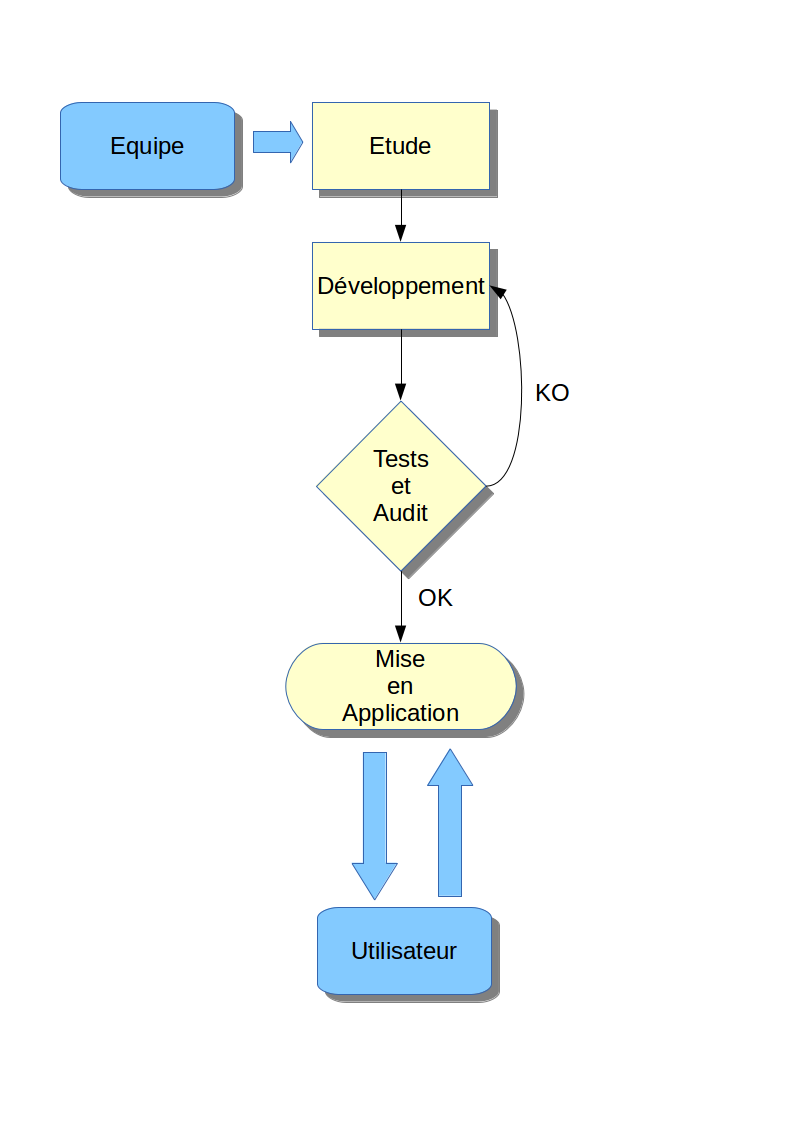
\includegraphics[scale=0.5]{../graphics/diagramme1.png}
  \caption{Sch\'{e}ma Macroscopique du Projet}
  \setlength{\parindent}{1cm}
  \begin{flushleft}
  Nous (l'�quipe) commencerons  par une \'{e}tude des diff\'{e}rents protocoles de g\'{e}n\'{e}rations d'OTP afin d'en fournir un \'{e}tat de l'art le plus exhaustif possible. Une fois celui-ci termin� nous passerons \`{a} l'impl\'{e}mentation des meilleurs protocoles retenues. Enfin, pour v\'{e}rifier notre production, un audit sera organis� ainsi qu'une batterie de tests de sorte \`{a} corriger les erreurs de d\'{e}veloppement pour nous mener \`{a} une mise en application. 
  \end{flushleft}
\end{figure}




\clearpage

\fiche{Association serveur-client-token}{Utilisateur}{Le serveur commnunique au Token un secret}{Il existe une communication client-serveur}{Bouton utilisateur}{Association r\'{e}ussie}{../graphics/association.jpg}{Impossible d'associer le token au serveur}
\\

\fiche{G\'{e}n\'{e}ration de l'OTP par le token}{Utilisateur}{L'utilisateur demande au token un nouvel OTP qui lui est retourn\'{e}}{Le token est li\'{e} au serveur}{L'utilisateur demande un OTP}{OTP g\'{e}n\'{e}r\'{e}}{../graphics/generation.jpg}{Null}
\\

\fiche{Authentification}{Utilisateur}{L'utilisateur tente de s'authentifier sur le serveur}{L'utilisateur poss�de un OTP}{L'utilisateur donne le mot de passe au serveur}{Utilisateur authentifi\'{e} ou rejet\'{e}}{../graphics/authentification.jpg}{Crash du serveur}
\\

\fiche{Re-Synchronisation}{Utilisateur}{Mise en accord du token et du serveur}{Il existe une connexion entre le token et le serveur}{Perte de la synchronisation}{Synchronisation retrouv\'{e}}{../graphics/resynchronisation.jpg}{Ne peut pas re-synchroniser}
\clearpage
\newpage
%-------------------------------------------------------------------------------
\section{Exigences op�rationnelles}
\begin{tabular}{|c|l|c|}
    \hline
    \rowcolor{gray}
    \textcolor{white}{Id} & \textcolor{white}{Intitul\'{e}} & \textcolor{white}{Priorit\'{e}}\\
    \hline
    EP\_01 & Le Token renvoie un OTP & Indispensable\\
    \hline
    EP\_02 & L'OTP est utilisable 1 seule fois & Indispensable\\
    \hline
    EP\_03 & L'OTP est non pr\'{e}visible (OTP qui ne peut \^{e}tre d\'{e}duit des anciens g�n�r�s) & Indispensable\\
    \hline
    EP\_04 & R\'{e}sistant � une attaque exhaustive & Indispensable\\
    \hline
    EP\_05 & R\'{e}sistant aux attaques par rejeu & Indispensable\\
    EP\_06 & Respect des RFC (RFC2289, RFC4226, RFC4256, RFC4793, RFC6238) & Indispensable\\
    \hline

    \hline
    
    
\end{tabular}

%-------------------------------------------------------------------------------
\section{Exigences d'interface}
\begin{tabular}{|c|l|c|}
    \hline
    \rowcolor{gray}
    \textcolor{white}{Id} & \textcolor{white}{Intitul\'{e}} & \textcolor{white}{Priorit\'{e}}\\
    \hline
    EI\_01 & UNIX(Client/Serveur/Token) & Indispensable\\
    \hline
    EI\_02 & Android(Token) & Important\\
    \hline
    EI\_03 & Java Card (Token) & Secondaire\\
    \hline
\end{tabular}

%-------------------------------------------------------------------------------
\section{Exigences de qualit�}
\begin{tabular}{|c|l|}
    \hline
    \rowcolor{gray}
    \textcolor{white}{Id} & \textcolor{white}{Intitul\'{e}}\\
    \hline
    EQ\_01 & G\'{e}n\'{e}ration de mots de passe inf\'{e}rieur � 1 seconde (sur un processeur cadenc\'{e} � 700MHz)\\
    \hline
    EQ\_02 & Temps de r\'{e}ponse serveur (temps < 1 sec + 2 *tps communication)\\
    \hline
    EQ\_03 & Le serveur supporte au moins 100 000 demandes de v\'{e}rification simultan\'{e}es\\
    \hline
    EQ\_04 & La v\'{e}rification est coh\'{e}rente\\
    \hline
    EQ\_05 & La g\'{e}n\'{e}ration utilise au plus 10 Ko de m\'{e}moire\\
    \hline
    EQ\_06 & \'{E}tat de l'art exhaustif, au moins trois protocoles OTP  \'{e}tudi\'{e}s\\
    \hline
\end{tabular}
%-------------------------------------------------------------------------------
\end{document}
